\documentclass[11pt,a4paper]{article}

\usepackage[T1]{fontenc}
\usepackage{lmodern}
\usepackage[margin=2.3cm]{geometry}
\usepackage{amsmath,amssymb}
\usepackage{booktabs}
\usepackage{graphicx}
\usepackage{float}
\usepackage{caption}
\usepackage{enumitem}
\usepackage{microtype}
\usepackage{xcolor}
\usepackage{fancyhdr}
\usepackage{listings}
\usepackage{tcolorbox}
\tcbuselibrary{breakable}
\usepackage{tikz}
\usetikzlibrary{arrows.meta,positioning,shapes.geometric,calc}
\usepackage[colorlinks=true,linkcolor=blue!50!black,urlcolor=blue!50!black,citecolor=blue!50!black]{hyperref}

\definecolor{accent}{RGB}{31,94,153}
\definecolor{warn}{RGB}{176,58,46}
\definecolor{codebg}{RGB}{246,248,250}

\newtcolorbox{keybox}[1][]{colback=accent!5,colframe=accent,fonttitle=\bfseries,title=#1,breakable}
\newtcolorbox{warnbox}[1][]{colback=warn!5,colframe=warn,fonttitle=\bfseries,title=#1,breakable}
\newtcolorbox{examplebox}[1][]{colback=green!4!white,colframe=green!40!black,fonttitle=\bfseries,title=#1,breakable}

\lstset{
  language=Python, basicstyle=\ttfamily\small, backgroundcolor=\color{codebg},
  keywordstyle=\color{accent}\bfseries, commentstyle=\color{gray}\itshape,
  stringstyle=\color{green!40!black}, frame=single, rulecolor=\color{gray!40},
  breaklines=true, showstringspaces=false, columns=fullflexible, numbers=left,
  numberstyle=\tiny\color{gray}
}

\pagestyle{fancy}
\fancyhf{}
\fancyhead[L]{\small MODWT Explained}
\fancyhead[R]{\small \nouppercase{\leftmark}}
\fancyfoot[C]{\thepage}

\setlength{\parskip}{0.45em}
\setlength{\parindent}{0pt}
\captionsetup{font=small,labelfont=bf}

\newcommand{\hwav}{\tilde{h}}
\newcommand{\gsc}{\tilde{g}}

\begin{document}

\begin{titlepage}
  \centering
  \vspace*{3cm}
  {\Huge\bfseries The Maximal Overlap\\[0.3em] Discrete Wavelet Transform\par}
  \vspace{0.8cm}
  {\Large An in-depth explanation with worked examples\par}
  \vspace{0.4cm}
  {\large Theory, hand calculations, properties and its role in WaveCatBoost\par}
  \vspace{2cm}
  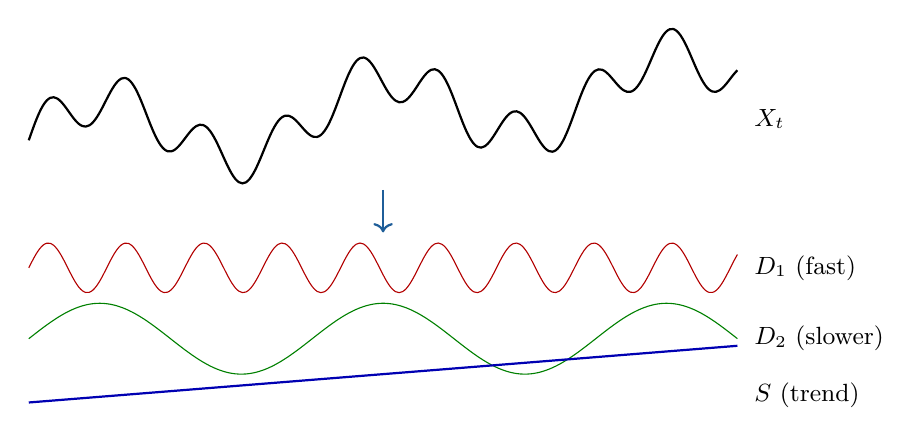
\begin{tikzpicture}[scale=0.9]
    \draw[thick] plot[smooth, domain=0:10, samples=200] (\x, {1.6+0.35*sin(\x*360/1.1)+0.5*sin(\x*360/4)+0.08*\x});
    \draw[->,thick,accent] (5,0.9) -- (5,0.3);
    \draw[red!70!black] plot[smooth, domain=0:10, samples=200] (\x, {-0.2+0.35*sin(\x*360/1.1)});
    \draw[green!50!black] plot[smooth, domain=0:10, samples=200] (\x, {-1.2+0.5*sin(\x*360/4)});
    \draw[blue!70!black, thick] plot[domain=0:10] (\x, {-2.1+0.08*\x});
    \node[right] at (10.1,1.9) {\small $X_t$};
    \node[right] at (10.1,-0.2) {\small $D_1$ (fast)};
    \node[right] at (10.1,-1.2) {\small $D_2$ (slower)};
    \node[right] at (10.1,-2.0) {\small $S$ (trend)};
  \end{tikzpicture}
  \vfill
  {\large Companion notes for the paper\\[0.2em]
  \emph{A Novel Hybrid Approach for Efficiently Forecasting Air Quality Data} (WaveCatBoost),\\
  IEEE Sensors Letters, 2025\par}
  \vspace{1cm}
\end{titlepage}

\tableofcontents
\newpage

%==========================================================================
\section{Why decompose a time series at all?}
%==========================================================================

An hourly air-quality series such as PM$_{2.5}$ is a superposition of behaviours that live on
very different time scales:

\begin{itemize}[leftmargin=1.5em]
  \item \textbf{Very fast variation}: sensor noise and sudden spikes (a passing truck, a fire), lasting an hour or two.
  \item \textbf{Intra-day structure}: morning and evening traffic peaks, the 12-hour and 24-hour cycles driven by traffic and boundary-layer meteorology.
  \item \textbf{Multi-day structure}: weather systems, weekday/weekend differences.
  \item \textbf{Slow trend}: seasonal build-up of pollution, long-term drift.
\end{itemize}

A single forecasting model fed with the raw series must learn all of these at once, even though
they follow very different dynamics. The idea behind wavelet-based hybrid forecasting is:

\begin{keybox}[The divide-and-conquer principle]
Split the series into components that each contain \emph{one} time scale, forecast each component
with its own model, then add the component forecasts back together.
\[
  X_t \;\xrightarrow{\text{MODWT}}\; \{D_{1,t},\dots,D_{J,t},S_{J,t}\}
  \;\xrightarrow{\text{forecast each}}\; \{\hat D_{1},\dots,\hat D_{J},\hat S_{J}\}
  \;\xrightarrow{\text{combine}}\; \hat X .
\]
\end{keybox}

\subsection{Why not just use the Fourier transform?}

The Fourier transform writes a signal as a sum of sines and cosines that extend over the
\emph{entire} record. It tells you \emph{which} frequencies are present but not \emph{when} they occur.
A pollution spike at hour 150 is spread across all Fourier coefficients, and a daily cycle whose
amplitude changes from summer to winter is described only by its average amplitude.
Air-quality series are \textbf{non-stationary}: their mean, variance and periodic structure
change over time. We need a tool that is localised in \emph{both} time and scale. That tool is the
wavelet transform.

%==========================================================================
\section{Wavelet fundamentals}
%==========================================================================

\subsection{What is a wavelet?}

A wavelet $\psi(t)$ is a ``small wave'': a function that oscillates but dies out quickly. It satisfies
\[
  \int_{-\infty}^{\infty}\psi(t)\,dt = 0 \qquad\text{(it has zero mean, so it measures \emph{change})},
  \qquad
  \int_{-\infty}^{\infty}\psi^2(t)\,dt = 1 .
\]
By \emph{stretching} the wavelet we look at slow changes, by \emph{squeezing} it we look at fast changes,
and by \emph{sliding} it along the time axis we locate those changes in time.

The simplest wavelet, and the one used in WaveCatBoost, is the \textbf{Haar wavelet}:
\[
  \psi^{\text{Haar}}(t) =
  \begin{cases}
    +1, & 0 \le t < \tfrac12,\\
    -1, & \tfrac12 \le t < 1,\\
    \phantom{+}0, & \text{otherwise.}
  \end{cases}
\]
Correlating a signal with a Haar wavelet simply computes ``(average of the recent half) minus (average of the
older half)''. It is a \emph{change detector}.

\subsection{From functions to filters}

For discrete data (one value per hour) we never use $\psi(t)$ directly. Instead we use two short
digital filters:

\begin{itemize}[leftmargin=1.5em]
  \item the \textbf{wavelet filter} $\{h_l\}_{l=0}^{L-1}$: a \emph{high-pass} filter that extracts detail (change);
  \item the \textbf{scaling filter} $\{g_l\}_{l=0}^{L-1}$: a \emph{low-pass} filter that extracts the smooth part (local average).
\end{itemize}

A valid (orthonormal) wavelet filter must satisfy
\begin{align}
  \sum_{l} h_l &= 0 && \text{(zero mean: a constant signal has no detail)} \label{eq:zero}\\
  \sum_{l} h_l^2 &= 1 && \text{(unit energy)} \label{eq:unit}\\
  \sum_{l} h_l\,h_{l+2n} &= 0 \quad (n\neq 0) && \text{(orthogonal to its even shifts)} \label{eq:orth}
\end{align}
and the scaling filter is obtained from it by the \emph{quadrature mirror} relation
$g_l = (-1)^{l+1}h_{L-1-l}$. Condition~\eqref{eq:orth} is the orthogonality relation that appears in the
WaveCatBoost paper (written there as $\sum_m p_m p_{m+2n}=0$ with $p$ the wavelet filter and $q$ the scaling filter).

\begin{examplebox}[Example: the Haar filters]
For Haar, $L=2$ and
\[
  h = \Big(\tfrac{1}{\sqrt2},\,-\tfrac{1}{\sqrt2}\Big), \qquad g = \Big(\tfrac{1}{\sqrt2},\,\tfrac{1}{\sqrt2}\Big).
\]
Check: $\tfrac{1}{\sqrt2}-\tfrac{1}{\sqrt2}=0$ \checkmark, \;
$\tfrac12+\tfrac12=1$ \checkmark. With $L=2$ there are no nonzero even shifts that overlap, so~\eqref{eq:orth} holds trivially.
Applied to a pair $(X_{t-1},X_t)$:
\[
  \text{wavelet: }\tfrac{1}{\sqrt2}(X_t - X_{t-1}) \quad\text{(a difference)},\qquad
  \text{scaling: }\tfrac{1}{\sqrt2}(X_t + X_{t-1}) \quad\text{(a scaled average)}.
\]
\end{examplebox}

%==========================================================================
\section{The ordinary DWT and its problems}
%==========================================================================

The classical \textbf{discrete wavelet transform} (DWT) uses Mallat's \emph{pyramid algorithm}:
filter the series with $h$ and $g$, then \textbf{keep only every second value} (downsample by 2). The
smooth half is fed into the next level and the process repeats. For Haar, level 1 is
\[
  W^{\text{DWT}}_{1,k} = \frac{X_{2k+1}-X_{2k}}{\sqrt2},\qquad
  V^{\text{DWT}}_{1,k} = \frac{X_{2k+1}+X_{2k}}{\sqrt2},\qquad k=0,\dots,\tfrac N2 - 1 .
\]
Each level halves the number of coefficients, so $N$ values become $N/2+N/4+\dots$ coefficients, $N$ in total.
That is efficient for compression, but it causes three problems for time-series forecasting:

\begin{enumerate}[leftmargin=1.5em]
  \item \textbf{Length restriction.} A level-$J$ DWT needs $N$ to be a multiple of $2^J$.
  \item \textbf{Shift variance.} Because pairs are formed as $(X_0,X_1),(X_2,X_3),\dots$, starting the series one
        hour later changes the pairing and therefore changes the coefficients \emph{completely},
        not just by a shift (see Section~\ref{sec:shift}).
  \item \textbf{Misalignment with time.} The level-$j$ coefficients are spaced $2^j$ hours apart, so they do not line up
        with the original hourly time axis. You cannot build lag features such as $D_{j,t-1}, D_{j,t-2}$ that are
        synchronised with $X_t$.
\end{enumerate}

The MODWT removes all three problems by \emph{not downsampling}.

%==========================================================================
\section{The MODWT: definition}
%==========================================================================

\subsection{Rescaled filters}

Because nothing is thrown away, the filters must be rescaled to keep energy balanced. The MODWT
filters are
\[
  \boxed{\;\hwav_l = \frac{h_l}{\sqrt2},\qquad \gsc_l = \frac{g_l}{\sqrt2}\;}
  \qquad\text{so for Haar:}\qquad
  \hwav = \big(\tfrac12,\,-\tfrac12\big),\quad \gsc = \big(\tfrac12,\,\tfrac12\big).
\]

\subsection{The MODWT pyramid algorithm}

Start with $V_{0,t}=X_t$. For each level $j=1,2,\dots,J$ compute, for \emph{every} $t=0,\dots,N-1$,
\begin{equation}
  \boxed{
  W_{j,t} = \sum_{l=0}^{L-1}\hwav_l\,V_{j-1,\,(t-2^{j-1}l)\bmod N},
  \qquad
  V_{j,t} = \sum_{l=0}^{L-1}\gsc_l\,V_{j-1,\,(t-2^{j-1}l)\bmod N}.}
  \label{eq:pyramid}
\end{equation}

Three things are worth noticing:
\begin{itemize}[leftmargin=1.5em]
  \item \textbf{No downsampling}: every level has exactly $N$ coefficients, one per time point.
  \item \textbf{Growing gaps}: at level $j$ the filter taps are $2^{j-1}$ steps apart (1, 2, 4, 8, \dots). This is the
        \emph{\`a trous} (``with holes'') trick: it is equivalent to inserting $2^{j-1}-1$ zeros between the filter
        coefficients. That is how deeper levels see longer time spans.
  \item \textbf{Circular boundary}: indices are taken $\bmod\,N$, so the series is treated as if it wrapped around:
        $X_{-1}$ means $X_{N-1}$. This affects the first few coefficients of each level (Section~\ref{sec:boundary}).
\end{itemize}

\begin{figure}[H]
\centering
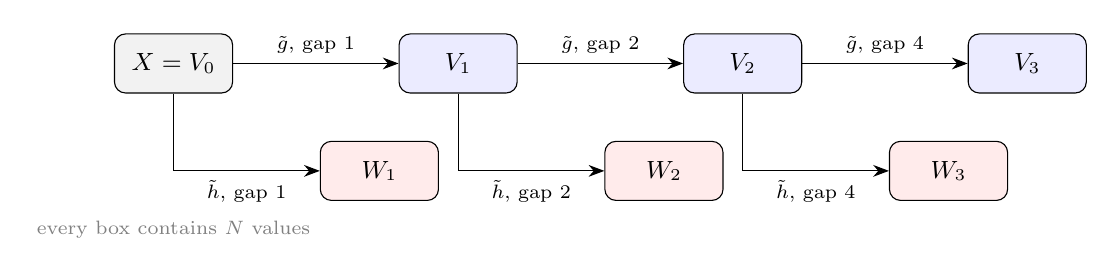
\begin{tikzpicture}[
  box/.style={draw,rounded corners,minimum width=1.5cm,minimum height=0.75cm,align=center,font=\small},
  wbox/.style={box,fill=red!8},
  vbox/.style={box,fill=blue!8},
  >={Stealth[length=2mm]}, node distance=0.9cm and 1.0cm]
  \node[box,fill=gray!10] (x) {$X=V_0$};
  \node[wbox,below right=0.6cm and 1.1cm of x] (w1) {$W_1$};
  \node[vbox,right=2.1cm of x] (v1) {$V_1$};
  \node[wbox,below right=0.6cm and 1.1cm of v1] (w2) {$W_2$};
  \node[vbox,right=2.1cm of v1] (v2) {$V_2$};
  \node[wbox,below right=0.6cm and 1.1cm of v2] (w3) {$W_3$};
  \node[vbox,right=2.1cm of v2] (v3) {$V_3$};
  \draw[->] (x) -- node[above,font=\scriptsize]{$\gsc$, gap 1} (v1);
  \draw[->] (x) |- node[pos=0.75,below,font=\scriptsize]{$\hwav$, gap 1} (w1);
  \draw[->] (v1) -- node[above,font=\scriptsize]{$\gsc$, gap 2} (v2);
  \draw[->] (v1) |- node[pos=0.75,below,font=\scriptsize]{$\hwav$, gap 2} (w2);
  \draw[->] (v2) -- node[above,font=\scriptsize]{$\gsc$, gap 4} (v3);
  \draw[->] (v2) |- node[pos=0.75,below,font=\scriptsize]{$\hwav$, gap 4} (w3);
  \node[font=\scriptsize,gray,below=1.5cm of x,align=left] {every box contains $N$ values};
\end{tikzpicture}
\caption{The MODWT pyramid. At each level the current smooth series is split into a detail series $W_j$ and a
smoother series $V_j$. The smooth series is split again, with the filter gap doubling each time.}
\label{fig:pyramid}
\end{figure}

\subsection{The Haar MODWT in plain words}

Plugging the Haar filters into~\eqref{eq:pyramid} gives very simple recursions:
\begin{equation}
  \boxed{
  W_{j,t} = \frac{V_{j-1,t} - V_{j-1,t-2^{j-1}}}{2},
  \qquad
  V_{j,t} = \frac{V_{j-1,t} + V_{j-1,t-2^{j-1}}}{2}.}
  \label{eq:haar}
\end{equation}

Unrolling the recursion gives an even more intuitive description. $V_{j,t}$ is the average of the
last $2^j$ observations, and $W_{j,t}$ is half the difference of two adjacent block averages:
\begin{align}
  V_{j,t} &= \frac{1}{2^j}\sum_{l=0}^{2^j-1} X_{t-l}, \label{eq:haarV}\\
  W_{j,t} &= \frac{1}{2}\Bigg[\underbrace{\frac{1}{2^{j-1}}\sum_{l=0}^{2^{j-1}-1}X_{t-l}}_{\text{mean of most recent }2^{j-1}}
            \;-\; \underbrace{\frac{1}{2^{j-1}}\sum_{l=2^{j-1}}^{2^{j}-1}X_{t-l}}_{\text{mean of the }2^{j-1}\text{ before that}}\Bigg].
  \label{eq:haarW}
\end{align}

\begin{keybox}[Intuition for the Haar MODWT]
\begin{itemize}[leftmargin=1.2em]
  \item $V_{j,t}$ is a moving average over a window of $2^j$ hours.
  \item $W_{j,t}$ is half the difference between two adjacent block averages, each $2^{j-1}$ hours long.
        It asks: \emph{did the level change between the previous block and the latest block?}
  \item $W_1$ compares single hours, $W_2$ compares 2-hour blocks, $W_3$ compares 4-hour blocks, and so on.
\end{itemize}
\end{keybox}

Equivalently, each level can be computed in one step with an \emph{equivalent filter} applied directly to $X$:
$W_{j,t} = \sum_l \hwav_{j,l}X_{t-l}$ and $V_{j,t}=\sum_l \gsc_{j,l}X_{t-l}$, where the equivalent filters have width
$L_j=(2^j-1)(L-1)+1$, which is $2^j$ for Haar. Figure~\ref{fig:filters} shows them.

\begin{figure}[H]
  \centering
  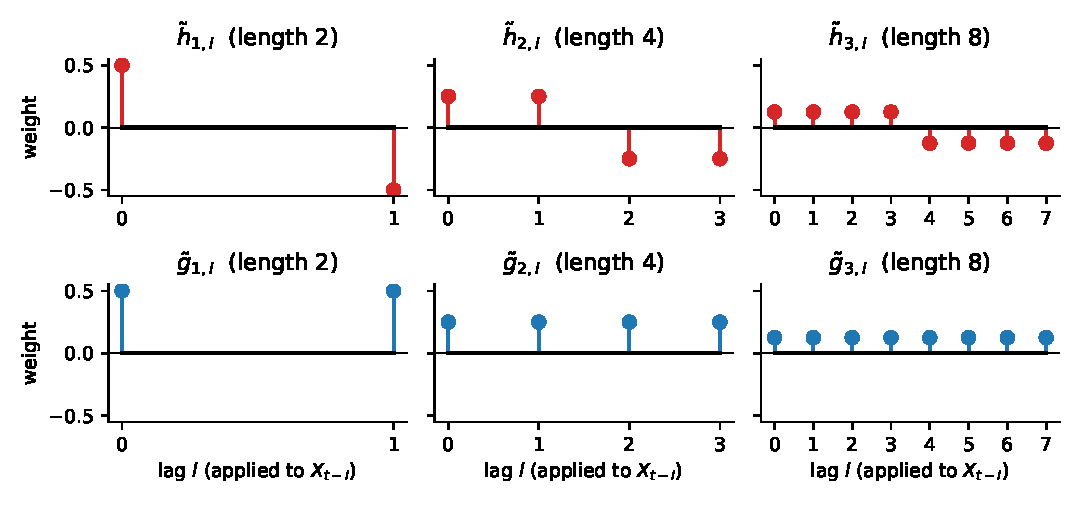
\includegraphics[width=\linewidth]{figs/haar_filters.pdf}
  \caption{Equivalent Haar MODWT filters for levels 1--3. The wavelet filters (top) are ``$+$block, $-$block''
  change detectors of growing width. The scaling filters (bottom) are plain moving averages of width $2^j$.}
  \label{fig:filters}
\end{figure}

%==========================================================================
\section{Worked example: computing the MODWT by hand}
\label{sec:example}
%==========================================================================

Take $N=8$ hourly PM$_{2.5}$ readings ($\mu$g/m$^3$) and decompose to $J=3$ levels with the Haar MODWT:
\[
  X = (20,\;22,\;25,\;24,\;28,\;30,\;27,\;26), \qquad t=0,\dots,7 .
\]
Entries marked $^{\ast}$ use the circular wrap-around (e.g.\ $X_{-1}=X_7=26$).

\subsection{Level 1: gap of 1 hour}

Apply~\eqref{eq:haar} with $j=1$: compare each value with the previous one.

\begin{table}[H]
\centering
\begin{tabular}{cccccc}
\toprule
$t$ & $X_t$ & $X_{t-1}$ & $W_{1,t}=\frac{X_t-X_{t-1}}{2}$ & $V_{1,t}=\frac{X_t+X_{t-1}}{2}$ & $W_{1,t}+V_{1,t}$ \\
\midrule
0 & 20 & 26$^{\ast}$ & $-3$ & 23 & 20 \\
1 & 22 & 20 & 1 & 21 & 22 \\
2 & 25 & 22 & 1.5 & 23.5 & 25 \\
3 & 24 & 25 & $-0.5$ & 24.5 & 24 \\
4 & 28 & 24 & 2 & 26 & 28 \\
5 & 30 & 28 & 1 & 29 & 30 \\
6 & 27 & 30 & $-1.5$ & 28.5 & 27 \\
7 & 26 & 27 & $-0.5$ & 26.5 & 26 \\
\bottomrule
\end{tabular}
\caption{Level 1. Example: $W_{1,4}=(28-24)/2=2$ and $V_{1,4}=(28+24)/2=26$.}
\end{table}

Notice $W_{1,t}+V_{1,t}=X_t$ for every $t$: the original value has been split exactly into a ``change''
part and an ``average'' part. The large value $W_{1,0}=-3$ is an artefact of the wrap-around: it compares
$X_0=20$ with $X_7=26$, which are not really neighbours.

\subsection{Level 2: gap of 2 hours, applied to $V_1$}

Now we decompose the smooth series $V_1$, comparing values \textbf{two} steps apart.

\begin{table}[H]
\centering
\begin{tabular}{ccccc}
\toprule
$t$ & $V_{1,t}$ & $V_{1,t-2}$ & $W_{2,t}=\frac{V_{1,t}-V_{1,t-2}}{2}$ & $V_{2,t}=\frac{V_{1,t}+V_{1,t-2}}{2}$ \\
\midrule
0 & 23 & 28.5$^{\ast}$ & $-2.75$ & 25.75 \\
1 & 21 & 26.5$^{\ast}$ & $-2.75$ & 23.75 \\
2 & 23.5 & 23 & 0.25 & 23.25 \\
3 & 24.5 & 21 & 1.75 & 22.75 \\
4 & 26 & 23.5 & 1.25 & 24.75 \\
5 & 29 & 24.5 & 2.25 & 26.75 \\
6 & 28.5 & 26 & 1.25 & 27.25 \\
7 & 26.5 & 29 & $-1.25$ & 27.75 \\
\bottomrule
\end{tabular}
\caption{Level 2. Example: $W_{2,5}=(29-24.5)/2=2.25$ and $V_{2,5}=(29+24.5)/2=26.75$.}
\end{table}

Check against~\eqref{eq:haarV}: $V_{2,5}$ should be the mean of the last four observations,
$(30+28+24+25)/4 = 26.75$ \checkmark. And~\eqref{eq:haarW}: $W_{2,5}=\tfrac12\big[\tfrac{30+28}{2}-\tfrac{24+25}{2}\big]
=\tfrac12[29-24.5]=2.25$ \checkmark.

\subsection{Level 3: gap of 4 hours, applied to $V_2$}

\begin{table}[H]
\centering
\begin{tabular}{ccccc}
\toprule
$t$ & $V_{2,t}$ & $V_{2,t-4}$ & $W_{3,t}=\frac{V_{2,t}-V_{2,t-4}}{2}$ & $V_{3,t}=\frac{V_{2,t}+V_{2,t-4}}{2}$ \\
\midrule
0 & 25.75 & 24.75$^{\ast}$ & 0.5 & 25.25 \\
1 & 23.75 & 26.75$^{\ast}$ & $-1.5$ & 25.25 \\
2 & 23.25 & 27.25$^{\ast}$ & $-2$ & 25.25 \\
3 & 22.75 & 27.75$^{\ast}$ & $-2.5$ & 25.25 \\
4 & 24.75 & 25.75 & $-0.5$ & 25.25 \\
5 & 26.75 & 23.75 & 1.5 & 25.25 \\
6 & 27.25 & 23.25 & 2 & 25.25 \\
7 & 27.75 & 22.75 & 2.5 & 25.25 \\
\bottomrule
\end{tabular}
\caption{Level 3. Example: $W_{3,7}=(27.75-22.75)/2=2.5$.}
\end{table}

$V_3$ is the mean of the last $2^3=8$ values. Since $N=8$ and the series is treated as circular, every
window contains all eight observations, so $V_{3,t}=202/8=25.25$ for all $t$: the coarsest smooth has
collapsed to the overall mean. In real applications $N\gg 2^J$ and $V_J$ is a genuine slowly varying trend.

\subsection{All coefficients together}

\begin{table}[H]
\centering
\begin{tabular}{ccccccc}
\toprule
$t$ & $X_t$ & $W_{1,t}$ & $W_{2,t}$ & $W_{3,t}$ & $V_{3,t}$ & $W_1{+}W_2{+}W_3{+}V_3$ \\
\midrule
0 & 20 & $-3$ & $-2.75$ & 0.5 & 25.25 & 20 \\
1 & 22 & 1 & $-2.75$ & $-1.5$ & 25.25 & 22 \\
2 & 25 & 1.5 & 0.25 & $-2$ & 25.25 & 25 \\
3 & 24 & $-0.5$ & 1.75 & $-2.5$ & 25.25 & 24 \\
4 & 28 & 2 & 1.25 & $-0.5$ & 25.25 & 28 \\
5 & 30 & 1 & 2.25 & 1.5 & 25.25 & 30 \\
6 & 27 & $-1.5$ & 1.25 & 2 & 25.25 & 27 \\
7 & 26 & $-0.5$ & $-1.25$ & 2.5 & 25.25 & 26 \\
\bottomrule
\end{tabular}
\caption{The complete Haar MODWT of $X$. Every row sums back to $X_t$.}
\label{tab:all}
\end{table}

Reading Table~\ref{tab:all}:
\begin{itemize}[leftmargin=1.5em]
  \item $W_1$ is small and erratic: hour-to-hour jitter.
  \item $W_2$ goes from negative ($t=0,1$) to positive ($t=3$--$6$): the series was rising over 2-hour blocks in the middle of the record.
  \item $W_3$ rises steadily from $-2.5$ to $+2.5$: the 4-hour block averages were climbing, which is the slower rise towards the peak at $t=5$.
  \item $V_3$ carries the overall level.
\end{itemize}

\begin{keybox}[A special property of Haar]
For the Haar wavelet, $\hwav+\gsc=(1,0)$, which implies $V_{j-1,t}=W_{j,t}+V_{j,t}$ at every level, and therefore
\[
  X_t = W_{1,t}+W_{2,t}+\dots+W_{J,t}+V_{J,t}.
\]
The coefficients themselves add up to the signal. This is \emph{not} true for longer wavelets (Daubechies,
least-asymmetric, \dots). For those you need the multiresolution analysis of Section~\ref{sec:mra}.
\end{keybox}

%==========================================================================
\section{Inverting the MODWT: perfect reconstruction}
%==========================================================================

The inverse MODWT (IMODWT) runs the pyramid backwards, from level $J$ down to level 1:
\begin{equation}
  V_{j-1,t} = \sum_{l=0}^{L-1}\hwav_l\,W_{j,(t+2^{j-1}l)\bmod N} + \sum_{l=0}^{L-1}\gsc_l\,V_{j,(t+2^{j-1}l)\bmod N},
  \qquad j=J,J-1,\dots,1,
  \label{eq:inverse}
\end{equation}
ending with $V_{0}=X$. Note the $+$ in the index: the inverse looks \emph{forward} in time. For Haar,
\[
  V_{j-1,t} = \tfrac12\big(W_{j,t} - W_{j,t+2^{j-1}}\big) + \tfrac12\big(V_{j,t} + V_{j,t+2^{j-1}}\big).
\]

\begin{examplebox}[Example: rebuilding $X_4$ from level 1]
From the level-1 table: $W_{1,4}=2$, $W_{1,5}=1$, $V_{1,4}=26$, $V_{1,5}=29$. Then
\[
  X_4 = \tfrac12(2-1) + \tfrac12(26+29) = 0.5 + 27.5 = 28 \;\checkmark
\]
\end{examplebox}

The inverse is exact: no information is lost by the MODWT. In WaveCatBoost this is the final
step. The forecasted coefficients are passed through the IMODWT to produce the forecast of the pollutant:
\[
  \hat X_{N+h} = \text{IMODWT}\big(\hat W_{1,N+h},\dots,\hat W_{J,N+h},\hat V_{J,N+h}\big).
\]

%==========================================================================
\section{Multiresolution analysis (MRA): details $D_j$ and smooth $S_J$}
\label{sec:mra}
%==========================================================================

The wavelet coefficients $W_j$ are \emph{measurements of change}. For interpretation and for an additive
decomposition that works with \emph{any} wavelet, we convert them back into the units of the original series.
The \textbf{detail} at level $j$ is what you get by inverting only $W_j$ (setting all other
coefficients to zero), and the \textbf{smooth} is what you get by inverting only $V_J$:
\[
  D_j = \text{IMODWT}(0,\dots,0,\underbrace{W_j}_{\text{level }j},0,\dots,0;\;0),
  \qquad
  S_J = \text{IMODWT}(0,\dots,0;\;V_J).
\]
Because the inverse is linear, these always add up exactly:
\begin{equation}
  \boxed{\;X_t = \sum_{j=1}^{J} D_{j,t} + S_{J,t}\;}
  \label{eq:mra}
\end{equation}
This is the decomposition written in the WaveCatBoost paper: $Y_t=\sum_{k=1}^K D_{k,t}+S_{K,t}$.

For Haar, the first detail is $D_{1,t}=\tfrac12(W_{1,t}-W_{1,t+1})$. It averages the change ``into'' $t$ with the
change ``out of'' $t$, which centres the detail on time $t$ (a \emph{zero-phase} filter).

\begin{table}[H]
\centering
\begin{tabular}{ccccccc}
\toprule
$t$ & $X_t$ & $D_{1,t}$ & $D_{2,t}$ & $D_{3,t}$ & $S_{3,t}$ & $D_1{+}D_2{+}D_3{+}S_3$ \\
\midrule
0 & 20 & $-2$ & $-1.875$ & $-1.375$ & 25.25 & 20 \\
1 & 22 & $-0.25$ & $-1.375$ & $-1.625$ & 25.25 & 22 \\
2 & 25 & 1 & $-0.375$ & $-0.875$ & 25.25 & 25 \\
3 & 24 & $-1.25$ & $-0.125$ & 0.125 & 25.25 & 24 \\
4 & 28 & 0.5 & 0.875 & 1.375 & 25.25 & 28 \\
5 & 30 & 1.25 & 1.875 & 1.625 & 25.25 & 30 \\
6 & 27 & $-0.5$ & 1.375 & 0.875 & 25.25 & 27 \\
7 & 26 & 1.25 & $-0.375$ & $-0.125$ & 25.25 & 26 \\
\bottomrule
\end{tabular}
\caption{Haar MRA of the example series. Example: $D_{1,0}=\tfrac12(W_{1,0}-W_{1,1})=\tfrac12(-3-1)=-2$.}
\label{tab:mra}
\end{table}

\subsection{Coefficients $W_j$ versus details $D_j$}

\begin{center}
\begin{tabular}{p{4.2cm}p{5cm}p{5cm}}
\toprule
 & \textbf{Wavelet coefficients} $W_{j,t}$ & \textbf{MRA details} $D_{j,t}$ \\
\midrule
What they measure & Change between block averages & The part of $X_t$ at scale $j$, in $\mu$g/m$^3$ \\
Time alignment & Lagged (filter looks backwards) & Centred on $t$ (zero phase) \\
Uses data from & $X_t, X_{t-1},\dots$ (past only) & Past \emph{and} future values \\
Adds up to $X$? & Only for Haar & Always \\
Energy preserved? & Yes (Section~\ref{sec:energy}) & Not in general \\
\bottomrule
\end{tabular}
\end{center}

The third row (``uses data from'') matters a great deal for forecasting. We return to it in Section~\ref{sec:leakage}.

%==========================================================================
\section{Key properties of the MODWT}
%==========================================================================

\subsection{Energy (variance) preservation}
\label{sec:energy}

The MODWT preserves energy:
\[
  \lVert X\rVert^2 = \sum_{j=1}^{J}\lVert W_j\rVert^2 + \lVert V_J\rVert^2 .
\]
So the total variability of the series can be split into contributions from each scale. This is called
the \textbf{wavelet variance}. For the example:

\begin{table}[H]
\centering
\begin{tabular}{lr}
\toprule
Quantity & Value \\
\midrule
$\lVert X\rVert^2$ & 5174 \\
$\lVert W_1\rVert^2$ & 20 \\
$\lVert W_2\rVert^2$ & 28 \\
$\lVert W_3\rVert^2$ & 25.5 \\
$\lVert V_3\rVert^2$ & 5100.5 \\
$\sum_j \lVert W_j\rVert^2 + \lVert V_3\rVert^2$ & 5174 \\
\bottomrule
\end{tabular}
\caption{Energy decomposition of the example. Almost all energy is in $V_3$ because the series has a large mean
(25.25). The fluctuating part has energy $20+28+25.5=73.5$, spread fairly evenly over the three scales.}
\end{table}

The wavelet variance tells you \emph{which time scales dominate} a pollutant's variability, which in turn
suggests how many levels to use and which components are hardest to forecast.

\subsection{Shift invariance}
\label{sec:shift}

If the input is shifted in time, the MODWT coefficients shift by the same amount and are otherwise unchanged.
The DWT does not have this property. Shift the example series circularly by one hour,
$X'=(26,20,22,25,24,28,30,27)$, and compare:

\begin{table}[H]
\centering
\begin{minipage}[t]{0.47\linewidth}\centering\small
\textbf{DWT}\par\smallskip
\begin{tabular}{ccc}
\toprule
$k$ & $W_{1,k}$ of $X$ & $W_{1,k}$ of $X'$ \\
\midrule
0 & 1.4142 & $-4.2426$ \\
1 & $-0.7071$ & 2.1213 \\
2 & 1.4142 & 2.8284 \\
3 & $-0.7071$ & $-2.1213$ \\
\bottomrule
\end{tabular}
\end{minipage}\hfill
\begin{minipage}[t]{0.47\linewidth}\centering\small
\textbf{MODWT}\par\smallskip
\begin{tabular}{ccc}
\toprule
$t$ & $W_{1,t}$ of $X$ & $W_{1,t}$ of $X'$ \\
\midrule
0 & $-3$ & $-0.5$ \\
1 & 1 & $-3$ \\
2 & 1.5 & 1 \\
3 & $-0.5$ & 1.5 \\
4 & 2 & $-0.5$ \\
5 & 1 & 2 \\
6 & $-1.5$ & 1 \\
7 & $-0.5$ & $-1.5$ \\
\bottomrule
\end{tabular}
\end{minipage}
\caption{$X'$ is $X$ shifted by one hour. Left: DWT level-1 coefficients change completely when the input is shifted by one hour.
Right: MODWT coefficients of the shifted series are simply the original coefficients moved down by one row.}
\end{table}

\begin{figure}[H]
  \centering
  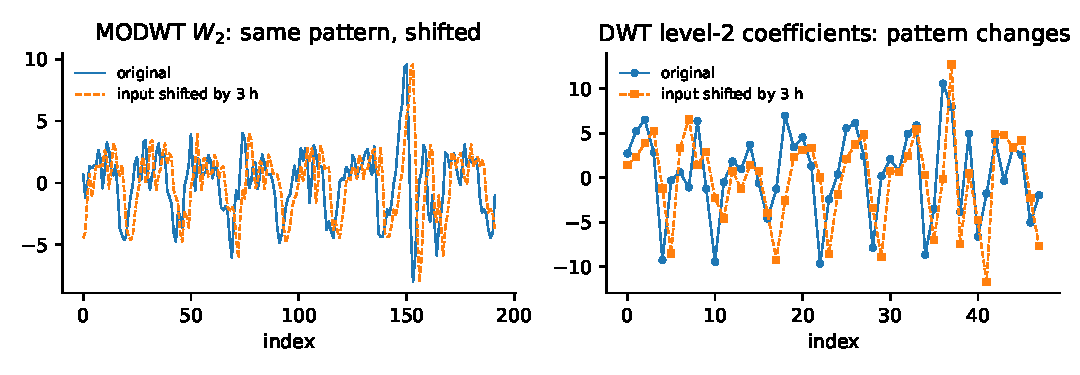
\includegraphics[width=\linewidth]{figs/shift_invariance.pdf}
  \caption{The same effect on a longer synthetic series shifted by 3 hours. The MODWT $W_2$ curves are identical
  apart from the shift. The DWT coefficients form a different pattern.}
\end{figure}

For forecasting, shift invariance means a pattern is described the same way no matter which hour it happens
to start at. A model trained on these features therefore sees consistent inputs.

\subsection{Works for any sample size}

The MODWT is defined for every $N$, not just multiples of $2^J$. The CPCB and ID1 series can be used as they are,
without trimming or padding.

\subsection{Redundancy}

A level-$J$ MODWT produces $(J+1)N$ numbers from $N$ observations. This redundancy is what buys
shift invariance and time alignment. The cost is $O(NJ)$ operations, which is negligible for hourly data.

\subsection{Boundary coefficients}
\label{sec:boundary}

Because of the circular treatment, the first $L_j-1$ coefficients of level $j$ mix the beginning of the series
with its end. For Haar, $L_j-1=2^j-1$: one coefficient at level 1, three at level 2, seven at level 3, and so on.
These are the starred entries in the worked example. With a year of hourly data ($N\approx 8760$) and $J=6$, only
the first 63 values are affected. They are usually discarded before training.

%==========================================================================
\section{Scale and frequency: what each level captures}
%==========================================================================

Each MODWT wavelet filter is a \textbf{band-pass} filter. Level $j$ is associated with the frequency band
\[
  \frac{1}{2^{j+1}} \le f \le \frac{1}{2^j}\quad\text{cycles per time step}
  \qquad\Longleftrightarrow\qquad
  \text{periods between } 2^j \text{ and } 2^{j+1} \text{ time steps.}
\]
The smooth $V_J$ (or $S_J$) holds everything with periods longer than $2^{J+1}$ steps.

\begin{figure}[H]
  \centering
  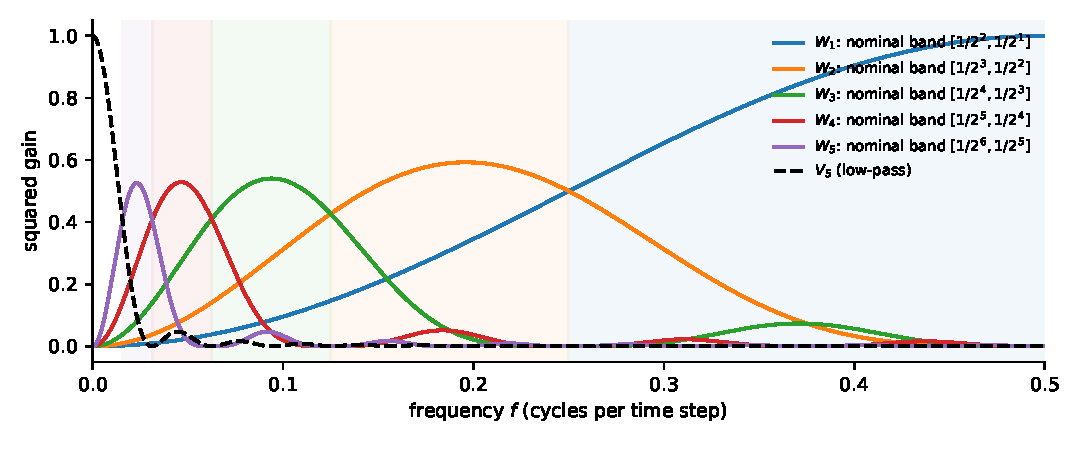
\includegraphics[width=\linewidth]{figs/haar_gain.pdf}
  \caption{Squared gain of the Haar MODWT filters for levels 1--5, with the nominal bands shaded. Each level passes
  roughly one octave of frequencies. Haar filters are short, so their bands overlap considerably. Longer
  wavelets give sharper bands.}
  \label{fig:gain}
\end{figure}

For \textbf{hourly} air-quality data this gives the following map:

\begin{table}[H]
\centering
\begin{tabular}{cclp{6.5cm}}
\toprule
Level & Physical scale $2^{j-1}$ & Periods captured & Typical air-quality content \\
\midrule
$D_1$ & 1 h & 2--4 h & sensor noise, short spikes \\
$D_2$ & 2 h & 4--8 h & rush-hour peaks, short events \\
$D_3$ & 4 h & 8--16 h & 12-hour (semi-diurnal) cycle \\
$D_4$ & 8 h & 16--32 h & \textbf{24-hour (diurnal) cycle} \\
$D_5$ & 16 h & 32--64 h & 2--3 day weather episodes \\
$D_6$ & 32 h & 64--128 h & synoptic weather systems \\
$S_6$ & -- & $>128$ h & weekly cycle (168 h), seasonal trend \\
\bottomrule
\end{tabular}
\caption{Interpretation of the MODWT levels for hourly data.}
\label{tab:levels}
\end{table}

\subsection{Choosing the number of levels $J$}

\begin{itemize}[leftmargin=1.5em]
  \item \textbf{Upper bound}: $2^J$ must be well below $N$, typically $J\le\lfloor\log_2 N\rfloor$ and in practice much smaller.
  \item \textbf{Physical reasoning}: choose $J$ so that the important cycles are separated. For hourly data, $J\ge4$ isolates
        the daily cycle in $D_4$.
  \item \textbf{Boundary cost}: each extra level doubles the number of boundary-affected points.
  \item \textbf{Model cost}: in WaveCatBoost, each level adds one CatBoost model.
\end{itemize}

%==========================================================================
\section{A realistic example: synthetic hourly PM$_{2.5}$}
%==========================================================================

To see the MODWT at work on something that looks like real data, we build a 32-day hourly series:
\[
  X_t = \underbrace{45+0.012t}_{\text{trend}}
  + \underbrace{9\sin\!\tfrac{2\pi(t-6)}{24} + 3.5\sin\!\tfrac{2\pi t}{12}}_{\text{daily and half-daily cycles}}
  + \underbrace{5\sin\!\tfrac{2\pi t}{168}}_{\text{weekly}}
  + \underbrace{\varepsilon_t}_{\text{noise},\;\sigma=2.5}
  + \underbrace{\text{3 short spikes}}_{\text{events}} .
\]

\begin{figure}[H]
  \centering
  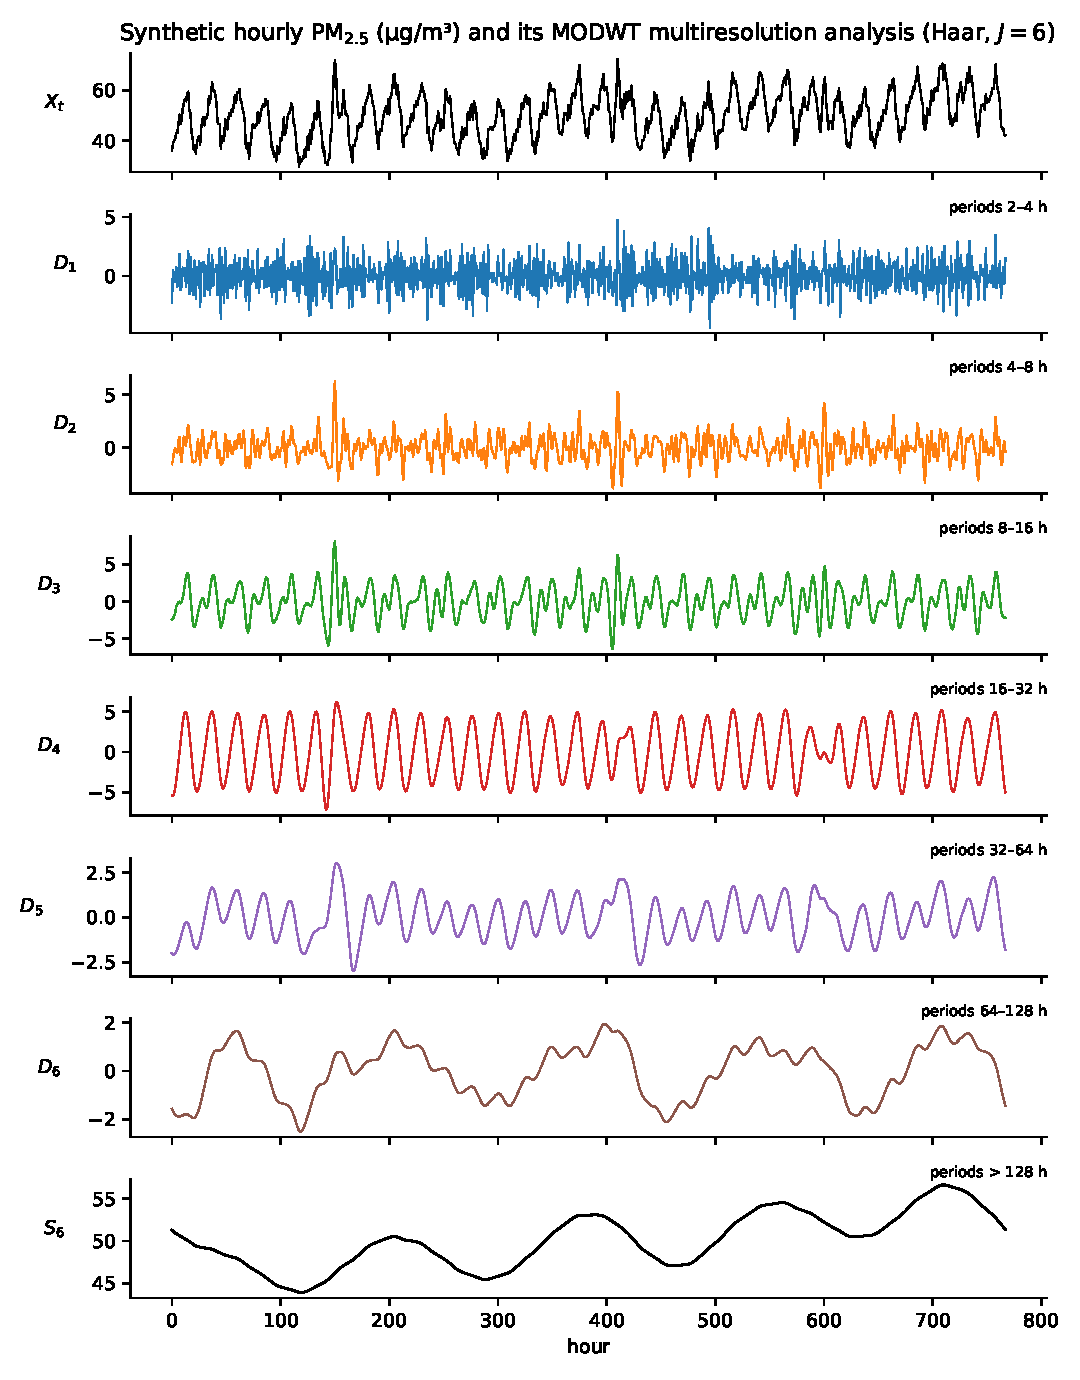
\includegraphics[width=\linewidth]{figs/synthetic_mra.pdf}
  \caption{Haar MODWT multiresolution analysis of the synthetic series ($J=6$). The components add up exactly to the top panel.}
  \label{fig:synmra}
\end{figure}

Reading Figure~\ref{fig:synmra} against Table~\ref{tab:levels}:
\begin{itemize}[leftmargin=1.5em]
  \item \textbf{$D_1$, $D_2$} contain the noise and the sharp parts of the three spikes (hours 150, 410, 600), which show up
        as localised bursts. The Fourier transform could not localise them in this way.
  \item \textbf{$D_3$} picks up the 12-hour cycle.
  \item \textbf{$D_4$} is dominated by a clean oscillation with a 24-hour period: the daily cycle.
  \item \textbf{$D_5$, $D_6$} contain leakage from neighbouring bands (Haar's bands overlap) and slow wiggles.
  \item \textbf{$S_6$} holds the weekly cycle riding on the upward trend.
\end{itemize}

\begin{figure}[H]
  \centering
  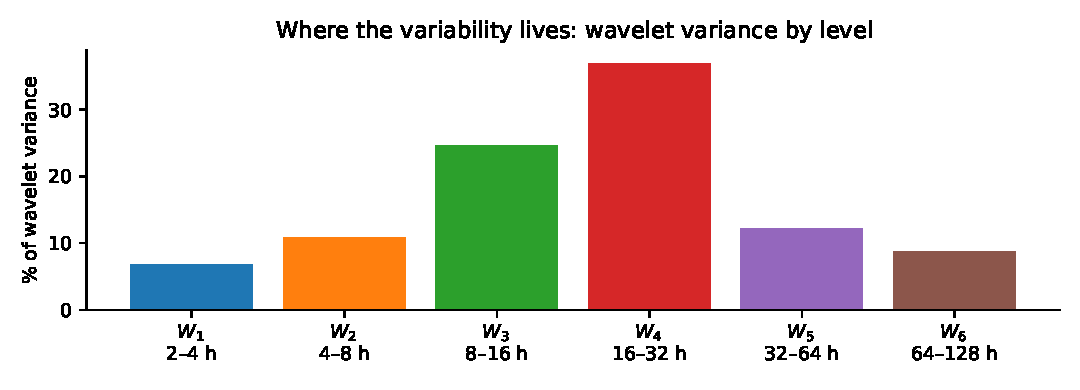
\includegraphics[width=\linewidth]{figs/synthetic_energy.pdf}
  \caption{Wavelet variance by level for the synthetic series. Level 4 dominates because the 24-hour cycle has the
  largest amplitude.}
\end{figure}

Each component is far simpler than $X_t$: $D_4$ is almost a sine wave, $S_6$ is smooth and slowly varying, and
$D_1$ is mostly noise. This is exactly why forecasting each component separately can beat forecasting $X_t$
directly.

%==========================================================================
\section{Choosing the wavelet}
%==========================================================================

\begin{center}
\begin{tabular}{p{3.2cm}p{5.4cm}p{5.4cm}}
\toprule
Wavelet & Advantages & Disadvantages \\
\midrule
Haar ($L=2$) & Simplest; shortest filter, so fewest boundary points; coefficients use only very recent data; coefficients add up to $X$ & Blocky; frequency bands overlap a lot \\
Daubechies D(4), D(6) & Smoother; better frequency separation & Longer filters, so more boundary points \\
Least asymmetric LA(8) & Near-linear phase, so features align well in time; common choice in time-series work & Filter length 8, so $L_j-1=7(2^j-1)$ boundary points \\
\bottomrule
\end{tabular}
\end{center}

WaveCatBoost uses Haar. The paper does not report an ablation over wavelet families, so trying D(4) or LA(8) would be
a natural experiment in a replication.

%==========================================================================
\section{MODWT inside WaveCatBoost}
%==========================================================================

\begin{figure}[H]
\centering
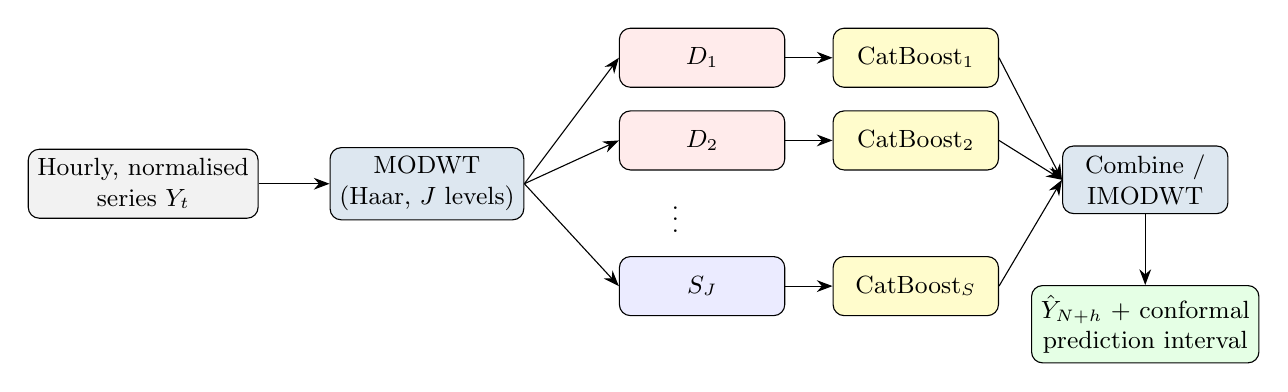
\begin{tikzpicture}[
  box/.style={draw,rounded corners,minimum height=0.75cm,align=center,font=\small,minimum width=2.1cm},
  >={Stealth[length=2mm]}]
  \node[box,fill=gray!10] (raw) {Hourly, normalised\\ series $Y_t$};
  \node[box,fill=accent!15,right=0.9cm of raw] (modwt) {MODWT\\(Haar, $J$ levels)};
  \node[box,fill=red!8,right=1.2cm of modwt,yshift=1.6cm] (d1) {$D_1$};
  \node[box,fill=red!8,right=1.2cm of modwt,yshift=0.55cm] (d2) {$D_2$};
  \node[font=\small,right=1.75cm of modwt,yshift=-0.35cm] (dots) {$\vdots$};
  \node[box,fill=blue!8,right=1.2cm of modwt,yshift=-1.3cm] (s) {$S_J$};
  \node[box,fill=yellow!20,right=0.6cm of d1] (c1) {CatBoost$_1$};
  \node[box,fill=yellow!20,right=0.6cm of d2] (c2) {CatBoost$_2$};
  \node[box,fill=yellow!20,right=0.6cm of s] (cs) {CatBoost$_S$};
  \node[box,fill=accent!15,right=0.8cm of c2,yshift=-0.5cm] (inv) {Combine /\\IMODWT};
  \node[box,fill=green!10,below=0.9cm of inv] (cp) {$\hat Y_{N+h}$ + conformal\\prediction interval};
  \draw[->] (raw) -- (modwt);
  \foreach \n in {d1,d2,s} \draw[->] (modwt.east) -- (\n.west);
  \draw[->] (d1) -- (c1); \draw[->] (d2) -- (c2); \draw[->] (s) -- (cs);
  \foreach \n in {c1,c2,cs} \draw[->] (\n.east) -- (inv.west);
  \draw[->] (inv) -- (cp);
\end{tikzpicture}
\caption{Role of the MODWT in WaveCatBoost.}
\end{figure}

\subsection{Step by step}

\begin{enumerate}[leftmargin=1.5em]
  \item \textbf{Decompose} the normalised series $Y_t$ into $D_{1,t},\dots,D_{J,t},S_{J,t}$.
  \item \textbf{Build lag features} for each component, which works because the MODWT keeps every component on the hourly time axis:
        \[
          \hat D_{j,t} = f_j\big(D_{j,t-1},D_{j,t-2},\dots,D_{j,t-p}\big),
          \qquad
          \hat S_{J,t} = f_S\big(S_{J,t-1},\dots,S_{J,t-p}\big),
        \]
        where each $f_j$ is a separate CatBoost regressor.
  \item \textbf{Forecast} each component recursively for $h = 24, 168, 336, 744$ steps (1, 7, 14, 31 days).
  \item \textbf{Reconstruct}: add the component forecasts (Haar / MRA) or apply the IMODWT (coefficients).
  \item \textbf{Quantify uncertainty} around $\hat Y$ with conformal prediction.
\end{enumerate}

\begin{examplebox}[Toy forecast]
Suppose that, for the next hour, the component models predict $\hat D_1=0.8$, $\hat D_2=1.4$, $\hat D_3=1.1$ and $\hat S_3=26.0$.
With an additive (MRA) decomposition the forecast is simply
$\hat X = 0.8+1.4+1.1+26.0 = 29.3\;\mu$g/m$^3$. Each model had an easier job: $\hat S_3$ only needs to follow a smooth
level, and $\hat D_1$ only needs to predict small hour-to-hour jitter. (These numbers are illustrative only and are not taken from the paper.)
\end{examplebox}

\subsection{A critical pitfall: look-ahead leakage}
\label{sec:leakage}

\begin{warnbox}[Decomposing the full series before splitting causes leakage]
MRA details $D_{j,t}$ are computed with the inverse transform~\eqref{eq:inverse}, which looks \textbf{forward}
in time. If you decompose the entire dataset first and then split it into training and test sets, the training
features at time $t$ already contain information from $t+1, t+2,\dots$, including test-period values.
Reported accuracy can then be far better than anything achievable in real-time forecasting.
\end{warnbox}

The example below makes this concrete. We compute the level-$j$ value at $t=6$ twice: once using the full series
$X_0,\dots,X_7$, and once using only the data available at that moment, $X_0,\dots,X_6$.

\begin{table}[H]
\centering
\begin{tabular}{lcc}
\toprule
Value at $t=6$ & using $X_0,\dots,X_7$ (full) & using $X_0,\dots,X_6$ only \\
\midrule
$D_{1,6}$ & $-0.5$ & 1 \\
$D_{2,6}$ & 1.375 & 0.5625 \\
$D_{3,6}$ & 0.875 & 0.2656 \\
$W_{1,6}$ & $-1.5$ & $-1.5$ \\
$W_{2,6}$ & 1.25 & 1.25 \\
$W_{3,6}$ & 2 & 1.875 \\
\bottomrule
\end{tabular}
\caption{The MRA details at $t=6$ change when the future value $X_7$ is removed, so they depend on the future.
The Haar coefficients $W_{1,6}$ and $W_{2,6}$ do not change, because they only use past data. $W_{3,6}$ changes only
because level 3 needs 8 past values and just 7 exist, which triggers the circular boundary.}
\end{table}

\textbf{Safe practice for forecasting experiments:}
\begin{itemize}[leftmargin=1.5em]
  \item Split the data chronologically \emph{first}, then decompose only the training portion.
  \item For the test period, use a \textbf{rolling (expanding-window) decomposition}: at each forecast origin, decompose
        only the data observed so far and take the last values as features.
  \item Alternatively, use the Haar \emph{coefficients} $W_{j,t}$ and $V_{J,t}$, which are causal by~\eqref{eq:haarV}--\eqref{eq:haarW},
        and reconstruct with the IMODWT. Discard the first $2^J-1$ boundary-affected points.
\end{itemize}

%==========================================================================
\section{Implementation in Python}
%==========================================================================

\subsection{From scratch (Haar)}

The Haar MODWT needs only \texttt{numpy.roll}. The code below was used to produce the tables in this document.

\begin{lstlisting}
import numpy as np

def haar_modwt(x, J):
    """Circular Haar MODWT. Returns [W_1, ..., W_J] and V_J."""
    V = np.asarray(x, dtype=float)
    W = []
    for j in range(1, J + 1):
        s = 2 ** (j - 1)
        V_lag = np.roll(V, s)          # V_{j-1, t-s}
        W.append((V - V_lag) / 2)      # wavelet (detail) coefficients
        V = (V + V_lag) / 2            # scaling (smooth) coefficients
    return W, V

def haar_inverse_step(W_j, V_j, j):
    """Recover V_{j-1} from W_j and V_j."""
    s = 2 ** (j - 1)
    return (W_j - np.roll(W_j, -s) + V_j + np.roll(V_j, -s)) / 2

def haar_imodwt(W, V_J):
    V = V_J
    for j in range(len(W), 0, -1):
        V = haar_inverse_step(W[j - 1], V, j)
    return V

def haar_mra(x, J):
    """Details D_1..D_J and smooth S_J with x = sum(D) + S."""
    W, V_J = haar_modwt(x, J)
    zeros = [np.zeros_like(w) for w in W]
    D = [haar_imodwt(zeros[:j] + [W[j]] + zeros[j + 1:], np.zeros_like(V_J))
         for j in range(J)]
    S = haar_imodwt(zeros, V_J)
    return D, S

x = np.array([20, 22, 25, 24, 28, 30, 27, 26], dtype=float)
W, V3 = haar_modwt(x, 3)
print(W[0])   # [-3.  1.  1.5 -0.5  2.  1. -1.5 -0.5]
print(V3)     # [25.25 25.25 ... 25.25]
\end{lstlisting}

\subsection{With PyWavelets}

PyWavelets implements the same decomposition through its stationary wavelet transform. We checked that the
following gives results identical to \texttt{haar\_mra} above:

\begin{lstlisting}
import pywt
components = pywt.mra(x, "haar", level=3, transform="swt")
S3, D3, D2, D1 = components      # ordered from coarsest to finest
\end{lstlisting}

In R, the \texttt{waveslim} package (\texttt{modwt}, \texttt{mra}) and the \texttt{wavelets} package
(\texttt{modwt}, \texttt{mra}) implement the transform as defined by Percival and Walden.

%==========================================================================
\section{Summary}
%==========================================================================

\begin{keybox}[MODWT cheat sheet]
\begin{itemize}[leftmargin=1.2em]
  \item \textbf{What}: a wavelet transform that splits a series into $J$ detail components and one smooth component,
        each the same length as the original.
  \item \textbf{How}: repeatedly filter the smooth series with a high-pass $\hwav$ and low-pass $\gsc$ filter, doubling the
        gap between filter taps at each level. There is no downsampling.
  \item \textbf{Haar version}: $W_{j,t}=\tfrac12(V_{j-1,t}-V_{j-1,t-2^{j-1}})$, \; $V_{j,t}=\tfrac12(V_{j-1,t}+V_{j-1,t-2^{j-1}})$.
  \item \textbf{Additive}: $X_t=\sum_j D_{j,t}+S_{J,t}$ exactly; for Haar, also $X_t=\sum_j W_{j,t}+V_{J,t}$.
  \item \textbf{Energy}: $\lVert X\rVert^2=\sum_j\lVert W_j\rVert^2+\lVert V_J\rVert^2$, which gives a variance-by-scale breakdown.
  \item \textbf{Scales}: level $j$ holds periods of $2^j$ to $2^{j+1}$ steps; for hourly data, $D_4$ holds the daily cycle.
  \item \textbf{Advantages over the DWT}: any $N$, shift invariant, time-aligned components, suited to lag features.
  \item \textbf{Watch out for}: circular boundary effects ($2^j-1$ points per level for Haar) and look-ahead leakage when MRA
        details are computed on the full dataset.
\end{itemize}
\end{keybox}

\section*{References}
\addcontentsline{toc}{section}{References}

\begin{enumerate}[label={[\arabic*]},leftmargin=2em]
  \item D.~B. Percival and A.~T. Walden, \emph{Wavelet Methods for Time Series Analysis}. Cambridge University Press, 2000.
        (The standard reference for the MODWT; Chapter 5 covers the definitions used here.)
  \item S.~Mallat, \emph{A Wavelet Tour of Signal Processing}, 3rd ed. Academic Press, 2008.
  \item J.~Borah, T.~Chakraborty, M.~S.~M. Nadzir, M.~G. Cayetano, F.~Benedetto and S.~Majumdar,
        ``A Novel Hybrid Approach for Efficiently Forecasting Air Quality Data (WaveCatBoost),''
        \emph{IEEE Sensors Letters}, 2025.
  \item G.~R. Lee \emph{et al.}, ``PyWavelets: A Python package for wavelet analysis,''
        \emph{Journal of Open Source Software}, 4(36), 1237, 2019.
\end{enumerate}

\end{document}
